\documentclass{article}

\usepackage{amsmath,amssymb}
\usepackage{tikz}
\usepackage{pgfplots}
\usepackage{xcolor}
\usepackage[left=2.1cm,right=3.1cm,bottom=3cm,footskip=0.75cm,headsep=0.5cm]{geometry}
\usepackage{enumerate}
\usepackage{enumitem}
\usepackage{marvosym}
\usepackage{tabularx}
\usepackage{multirow}

\usepackage[utf8]{inputenc}

\renewcommand*{\arraystretch}{1.4}

\newcolumntype{L}[1]{>{\raggedright\arraybackslash}p{#1}}
\newcolumntype{R}[1]{>{\raggedleft\arraybackslash}p{#1}}
\newcolumntype{C}[1]{>{\centering\let\newline\\\arraybackslash\hspace{0pt}}m{#1}}

\title{\textbf{Rechtfertigung der Staatstätigkeit, Hausaufgabe 4}}
\author{\textsc{Henry Haustein}}
\date{}

\begin{document}
	\maketitle
	
	\section*{Aufgabe 1}
	\begin{enumerate}[label=(\alph*)]
		\item Es gilt Angebot = Nachfrage, wobei wir die Angebotsfunktion noch in die Form $p(x)$ bringen müssen: $p(x)=x+6$. Dann gilt
		\begin{align}
			x+6 &= 16-2x \notag \\
			x^{priv} &= \frac{10}{3} \Rightarrow p^{priv}=\frac{28}{3} \notag
		\end{align}
		\item Die sozialen Grenzkosten sind $GK^{soz}=GK + GS = 3x+6$ und damit gilt
		\begin{align}
			GK^{soz} &= GZB \notag \\
			3x+6 &= 16-2x \notag \\
			x^{opt} &= 2 \Rightarrow p^{opt}=12 \notag
		\end{align}
		\item Diagramm
		\begin{center}
			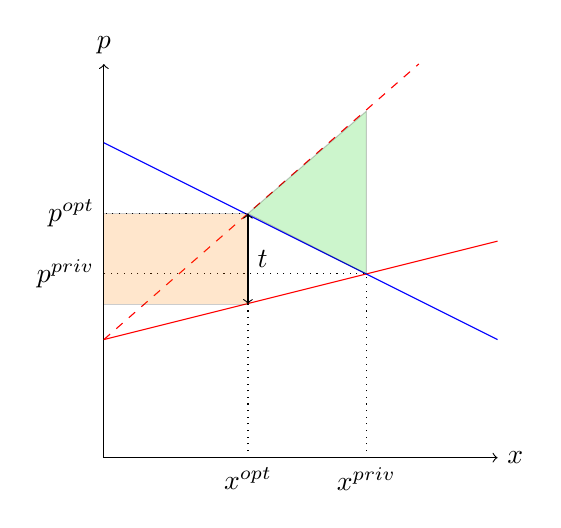
\begin{tikzpicture}
				\draw[->] (0,0) -- (5,0) node[right] {$x$};
				\draw[->] (0,0) -- (0,5) node[above] {$p$};
				
				\draw[red] (0,1.5) -- (5,11/4);
				\draw[red,dashed] (0,1.5) -- (4,5);
				\draw[blue] (0,4) -- (5,1.5);
				
				\draw[dotted] (10/3,0) node[below] {$x^{priv}$} -- (10/3,7/3) -- (0,7/3) node[left] {$p^{priv}$};
				\draw[dotted] (1.83,0) node[below] {$x^{opt}$} -- (1.83,3.1) -- (0,3.1) node[left] {$p^{opt}$};
				
				\draw[fill=green!80!black, opacity=0.2] (1.83,3.1) -- (10/3,7/3) -- (10/3,4.4) -- (1.83,3.1);
				\draw[fill=orange,opacity=0.2] (1.83,3.1) rectangle (0,1.95);
				\draw[<->] (1.83,1.95) to node[midway,right] {$t$} (1.83,3.1);
			\end{tikzpicture} \\
			\textcolor{blue}{GZB}, \textcolor{red}{GK bzw. soziale Grenzkosten}, \textcolor{green!80!black}{Wohlfahrtsverlust}, \textcolor{orange}{Steueraufkommen}
		\end{center}
		\item Da die Fabrik in der Laissez-faire-Lösung den Schaden den kollektiven Grenzschaden ignoriert, unterscheidet sich die kollektive von individuellen Optimallösung.
		\begin{align}
			WFV &= \frac{1}{2}(x^{priv}-x^{opt})(GK^{soz}(x^{priv}) - GK(x^{priv})) \notag \\
			&= \frac{1}{2}\left(\frac{10}{3}-2\right)\left(16-\frac{28}{3}\right) \notag \\
			&= \frac{40}{9} \notag
		\end{align}
		\item Die Steuer muss dem marginalen Umweltschaden in $x^{opt}$ entsprechen. Dieser ist
		\begin{align}
			t = GS(x^{opt}) = 2\cdot x^{opt} = 4 \notag
		\end{align}
		Das Steueraufkommen ist damit $2\cdot 4=8$.
		\item Da für die ersten Einheiten der kollektive Grenznutzen den kollektiven Grenzschaden übersteigt, profitiert die Gesellschaft stärker als sie unter dem Umweltschaden leidet.
		\item Vergleich der Produzentenrenten vor und nach Besteuerung:
		\begin{align}
			PR_{vor} &= \frac{1}{2}x^{priv}(p^{priv-6}) \notag \\
			&= \frac{1}{2}\cdot\frac{10}{3} - \frac{10}{3} \notag \\
			&= \frac{50}{3} \notag \\
			PR_{nach} &= \frac{1}{2}x^{opt}(p^{opt}-t-6) \notag \\
			&= \frac{1}{2}\cdot 2\cdot 2 \notag \\
			&= 2 \notag
		\end{align}
		Die Differenz ist $-\frac{32}{9}$.
		\item Für die einzelnen Fälle ergibt sich:
		\begin{itemize}
			\item Die Steuer bindet nicht in $x^{opt}$, es wird also $x^{priv}$ produziert. Die Steuerbelastung wird halbiert, es sinkt also auf 4.
			\item Die Steuer bindet in $x^{opt}$, damit wird auch $x^{opt}$ produziert. Zudem sinkt die Steuerlast auf 4.
			\item Es ergibt sich
			\begin{align}
				p &= GK + \frac{t}{2} \notag \\
				16-2x &= 6+x+2 \notag \\
				x &= \frac{8}{3} \notag
			\end{align}
			Die Produktion nähert sich $x^{opt}$ an, erreicht dieses aber nicht. Die Steuerbelastung sinkt auf $T=\frac{8}{3}\cdot 2=\frac{16}{3}$.
		\end{itemize}
	\end{enumerate}
	
	\section*{Aufgabe 2}
	\begin{enumerate}[label=(\alph*)]
		\item Die privaten Grenzkosten sind $GK^{priv}=2x$. Die sozialen Grenzkosten sind $GK^{soz}=GK^{priv} + GS = 2x + 20$. Die optimale Menge ist bei
		\begin{align}
			GK^{soz} &= p \notag \\
			2x^{opt} + 20 &= 50 \notag \\
			x^{opt} &= 15 \notag
		\end{align}
		Ohne staatlichen Eingriff wird
		\begin{align}
			GK^{priv} &= p \notag \\
			2x^{priv} &= 50 \notag \\
			x^{priv} &= 25 \notag
		\end{align}
		hergestellt.
		\item Der Wohlfahrtsverlust ist
		\begin{align}
			\frac{1}{2}(x^{priv} - x^{opt}) \cdot GS = \frac{1}{2}(25-15)\cdot 20 = 100 \notag
		\end{align}
		\item Diagramm
		\begin{center}
			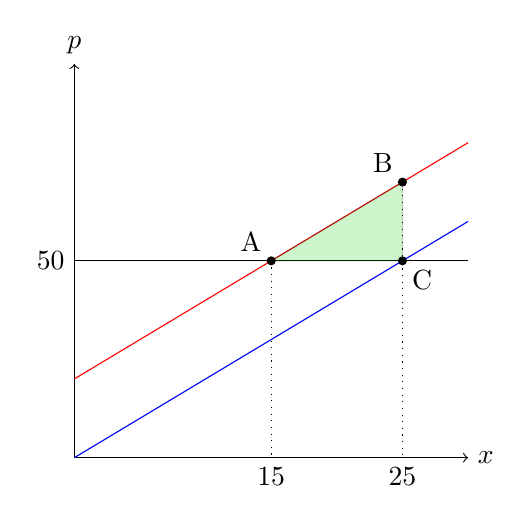
\begin{tikzpicture}
				\draw[->] (0,0) -- (5,0) node[right] {$x$};
				\draw[->] (0,0) -- (0,5) node[above] {$p$};
				
				\draw (0,2.5) node[left] {50} -- (5,2.5);
				\draw[blue] (0,0) -- (5,3);
				\draw[red] (0,1) -- (5,4);
				
				\draw[dotted] (4.167,3.5) -- (4.167,0) node[below] {25};
				\draw[dotted] (2.5,2.5) -- (2.5,0) node[below] {15};
				
				\draw[fill=green!80!black,opacity=0.2] (2.5,2.5) -- (4.167,3.5) -- (4.167,2.5) -- (2.5,2.5);
				
				\draw[fill=black] (4.167,2.5) circle (0.05) node[below right] {C};
				\draw[fill=black] (2.5,2.5) circle (0.05) node[above left] {A};
				\draw[fill=black] (4.167,3.5) circle (0.05) node[above left] {B};
			\end{tikzpicture} \\
			\textcolor{blue}{$GK^{priv}$}, \textcolor{red}{$GK^{soz}$}, \textcolor{green!80!black}{Wohlfahrtsverlust}
		\end{center}
		\item Die Pigou-Steuer soll die Kosten des Umweltschadens in $x^{opt}$ darstellen, also
		\begin{align}
			t &= GK^{soz}(x^{opt}) - GK^{priv}(x^{opt}) \notag \\
			&= (2\cdot 15+20) - (2\cdot 15) \notag \\
			&= 20 \notag
		\end{align}
		Das Steueraufkommen beträgt dann $x^{opt}\cdot t = 15\cdot 20 = 300$.
	\end{enumerate}
	
	\section*{Aufgabe 3}
	\begin{enumerate}[label=(\alph*)]
		\item Es gilt
		\begin{align}
			\begin{array}{lcl}
				GV_1 = 60-s_1 & \Rightarrow & s_1 = 60-GV_1 \\
				GV_2 = 60-2s_2 & \Rightarrow & s_2 = 30 - \frac{1}{2}GV_2 \\
				\cline{3-3}
				&&s\;\, = 90 - \frac{3}{2}GV
			\end{array} \notag
		\end{align}
		Also $GV = 60 - \frac{2}{3}s$.
		\item Es gilt
		\begin{align}
			\begin{array}{lcl}
				D_1 = \frac{1}{2}s^2 & \Rightarrow & GD_1 = s \\
				D_2 = \frac{1}{2}s^2 & \Rightarrow & GD_2 = s \\
				\cline{3-3}
				&&GD\;\, = 2s
			\end{array} \notag
		\end{align}
		\item Die Unternehmen kaufen solange ein, bis $GV=p$, also
		\begin{align}
			GV &= p \notag \\
			60-\frac{2}{3}s^{priv} &= 4 \notag \\
			s^{priv} &= 84 \notag
		\end{align}
		\item Mit der Samuelson-Regel folgt
		\begin{align}
			\sum GV_i &= \sum GN_j + p \notag \\
			GV &= GD \notag \\
			60-\frac{2}{3}s^{opt} &= 2s^{opt} + 4 \notag \\
			s^{opt} &= 21 \notag
		\end{align}
		\item Die Pigou-Steuer soll die Grenznachteile bei $s^{opt}$ aufwiegen, also
		\begin{align}
			t = GD(s^{opt}) = 2\cdot 21 = 42 \notag
		\end{align}
		\item Die Unternehmen teilen sich $s^{opt}$ so auf, dass $GV_1=GV_2$ unter der Nebenbedingung $s_1+s_2=21$ gilt:
		\begin{align}
			GV_1 &= GV_2 \notag \\
			60-s_1 &= 60-2\cdot (21-s_1) \notag \\
			s_1 &= 14 \notag \\
			s_2 &= 7 \notag
		\end{align}
	\end{enumerate}

	\section*{Aufgabe 4}
	\begin{enumerate}[label=(\alph*)]
		\item Unternehmen 1 handelt
		\begin{align}
			120-2s_1 &= 0 \notag \\
			s_1 &= 60 \notag
		\end{align}
		Unternehmen 2 handelt
		\begin{align}
			120-3s_2 &= 0 \notag \\
			s_2 &= 40 \notag
		\end{align}
		Es werden also 60 + 40 = 100 Schadstoffe ausgestoßen.
		\item Diagramm
		\begin{center}
			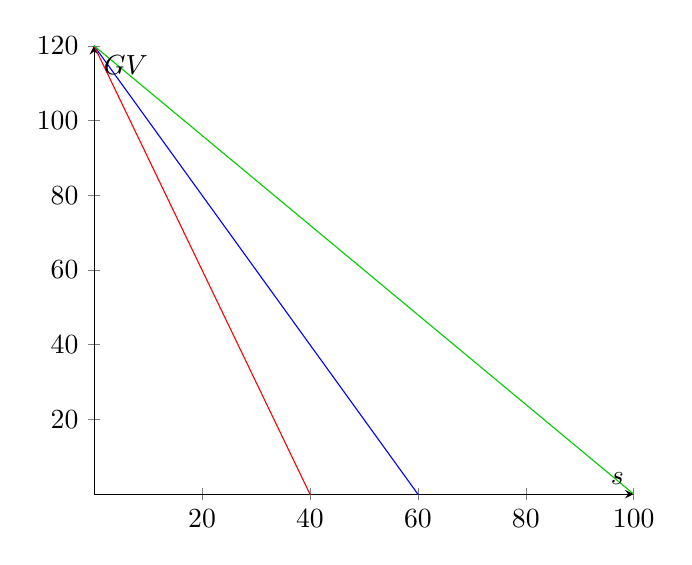
\begin{tikzpicture}
				\begin{axis}[
					xmin=0, xmax=100, xlabel=$s$,
					ymin=0, ymax=120, ylabel=$GV$,
					samples=400,
					axis x line=middle,
					axis y line=middle,
					domain=0:100,
					]
					\addplot[mark=none,smooth,blue] {120-2*x};
					\addplot[mark=none,smooth,red] {120-3*x};
					\addplot[mark=none,smooth,green!80!black] {120-6/5*x};
					
				\end{axis}
			\end{tikzpicture} \\
			\textcolor{blue}{$GV_1$}, \textcolor{red}{$GV_2$}, \textcolor{green!80!black}{$\sum GV_i$}
		\end{center}
		\item Es gilt $GV_1=GV_2$ und $s_1+s_2=80$, also
		\begin{align}
			GV_1 &= GV_2 \notag \\
			120-2(80-s_2) &= 120-3s_2 \notag \\
			s_2 &= 32 \Rightarrow s_1 = 48 \notag
		\end{align}
		\item Der Wohlfahrtsverlust kommt zustande, weil der Grenzvorteil von Firma 1 aus einer zusätzlichen Einheit zwischen $s_1^{opt}$ und 40 größer ist, als der marginale Nachteil von Firma 2 bei Verzicht auf eine Einheit.
		\begin{center}
			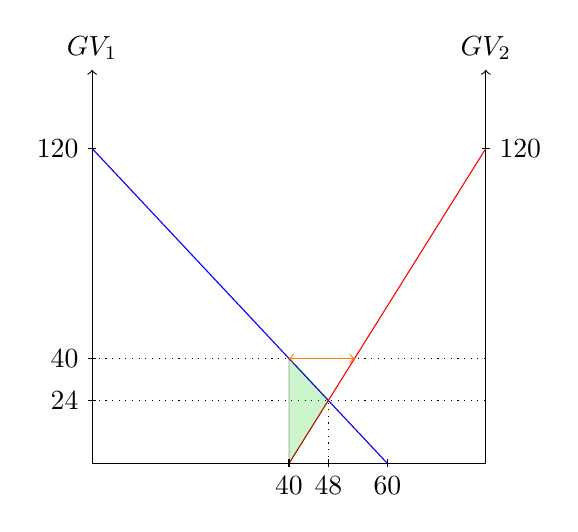
\begin{tikzpicture}
				\draw[->] (0,0) -- (0,5) node[above] {$GV_1$};
				\draw (0,0) -- (5,0);
				\draw[->] (5,0) -- (5,5) node[above] {$GV_2$};
				
				\draw[blue] (0,4) -- (3.75,0);
				\draw[red] (5,4) -- (2.5,0);
				
				\draw[dotted] (3,0) -- (3,0.8);
				\draw[dotted] (0,0.8) -- (5,0.8);
				\draw[dotted] (0,4/3) -- (5,4/3);
				
				\draw[fill=green!80!black,opacity=0.2] (2.5,0) -- (2.5,4/3) -- (3,0.8) -- (2.5,0);
				
				\draw[orange,<->] (2.5,4/3) -- (10/3,4/3);
				
				\draw (-0.05,4) node[left] {120} -- (0.05,4);
				\draw (-0.05,0.8) node[left] {24} -- (0.05,0.8);
				\draw (-0.05,4/3) node[left] {40} -- (0.05,4/3);
				\draw (4.95,4) -- (5.05,4) node[right] {120};
				\draw (2.5,0.05) -- (2.5,-0.05) node[below] {40};
				\draw (3.75,0.05) -- (3.75,-0.05) node[below] {60};
				\draw (3,0.05) -- (3,-0.05) node[below] {48};
			\end{tikzpicture} \\
			\textcolor{blue}{$GV_1$}, \textcolor{red}{$GV_2$}, \textcolor{green!80!black}{Wohlfahrtsverlust}
		\end{center}
		\begin{align}
			WFV &= \frac{1}{2}(s_1^{opt}-40)\cdot GV_1(40) \notag \\
			&= \frac{1}{2} \cdot 8\cdot 40 \notag \\
			&= 160 \notag
		\end{align}
		\item Wenn ein Zertifikat 40 kostet, kauft Firma 1:
		\begin{align}
			GV_1 &= 40 \notag \\
			120-2s_1 &= 40 \notag \\
			s_1 &= 40 \notag
		\end{align}
		Firma 2 kauft
		\begin{align}
			GV_2 &= 40  \notag \\
			120-3s_2 &= 40 \notag \\
			s_2 &= \frac{80}{3} \notag
		\end{align}
		Es werden weniger als 80 Zertifikate verkauft, die Umwelt ist also zu sauber (siehe \textcolor{orange}{oranger Pfeil} in (d)).
		\item analog zu (c). $s_1=48$, $s_2=32$ und $p=24$.
	\end{enumerate}

\end{document}